\chapter{\label{c:esd-concept}Infrastructure for the control of a plate capacitor electrostatic actuator with reduced seismic coupling}

\begin{itemize}
  \item Introduce Holger's paper~\cite{Wittel2015} \etal{}, discuss need for high voltages
  \item See AEI labbook p187 for discussion of AEI 100 g suspensions and why ESDs might be required. Hints of the equations to derive the response of the ESD to voltage applied across plates.
  \item Actuators usually couple noise, which is why magnets are usually on a stage above the test masses. This necessarily limits range, as any actuation performed by the magnets will be filtered by 1/f
  \item Immunity to seismic noise due to turning points on graph from Holger's paper (see C.G. talk)
  \item ESDs are useful in particular for this experiment because the mirror masses are small. Previously considered for GEO but the mirrors are too heavy for it to be effective.
  \item Test alignment couplings with ESD...
  \item This experiment will inform the main SSM experiment...
  \item HV amplifier design: pressure and temperature cut-offs (explanation of how it works), input/output signals, choice of connectors, routing of signals for ease of assembly (front panel disconnect, etc.)
  \item Protective earthing (how the removal of the ground supply from the GEO supply will clamp ground to Earth beyond 18 V)
  \item HV amplifier transfer functions
  \item HV amplifier noise measurement
  \item Resistor on output of amplifier design to limit current and damp resonant RCL modes: resistor adds loss, so lowers the Q associated with any suspension or cable pickups
  \item Amplifier incorporates low quiescent current (opposed to PA98) hence heat requirements, voltage range, whitening, cutoffs, soft start, quad channels.
  \item Discuss digital infrastructure: CDS digital I/O, avoiding ground loops, the DB25-37 converter board, pull-up resistors, etc.
\end{itemize}

\section{Electrostatic drives as actuators in suspended interferometer experiments}

\subsection{Electrostatic actuators in suspended interferometers}
Suspended test masses in interferometers require positional corrections in order for the interferometer to be kept at its operating point. This is typically provided via actuators on the suspension system, and predominantly involves voice coil actuators composing magnets and wound wire. Force noise can be introduced to the test masses by their actuators due to various effects such as electronic noise in the driver circuitry, Barkhausen noise \cite{Weiss2008} and seismic coupling via the actuator attachment point. The first two effects can usually be mitigated with appropriate design and shielding, for example by choosing appropriate electronic components and by making the magnets small and the electromagnetic environment quiet. The third effect is often mitigated by suspending the actuators from a separate suspension behind the test mass called a \emph{reaction} suspension. This provides seismic filtering to the actuators such that the ground motion coupling introduced to the test masses from the actuators is of similar magnitude to the ground motion the test masses would in any case receive with no actuation.

As introduced in Chapter\,\ref{c:speedmeter-control}, electrostatic drives (\glspl{ESD}) are a type of actuator employed in \GEO{} and \ALIGO{} for fast (high frequency) corrections to the interferometer. This actuator creates a force on a dielectric test mass by creating a potential difference between anodes and cathodes applied to the face of the reaction mass. Electromagnetic field gradients are then formed in such a way that the test mass can be pushed or pulled in a particular direction. The \gls{ESD} design used in the aforementioned detectors involves a comb of interlocking anodes and cathodes across which a voltage is applied to create the desired force. Alignment control is achieved through the use of multiple sets of combs on the face of the reaction mass, and the sign of the applied voltage can be controlled to induce torque.

There are a number of problems with this approach to low noise, high frequency actuation. There are obviously cost and technical implications to the use of a reaction suspension system behind each main suspension. The alignment of this second suspension must also be controlled and damped in the presence of displacement noise. With the use of \glspl{ESD}, the gap created between the reaction and test masses may also lead to \emph{squeezed film damping} due to residual gas in the vacuum system. One of the most fundamental considerations in the use of this \gls{ESD} design, however, is that it limits the clear aperture behind the test mass. The beam size on the \glspl{ETM} of \ALIGO{} is around \SI{6}{\centi\meter} and so in this case if the transmitted light were to be measured for the purposes of sensing and control the choice would have to be made between clipping of the beam and a reduction in the space available on the reaction mass for the electrostatic comb structure.

\subsection{Plate capacitor electrostatic drive design}
Applying a potential difference across metal plates effectively creates a capacitor. The electrostatic energy in the capacitor's field is given by the volume integral of the electric field created by the potential difference multiplied by the permittivity of the volume enclosed by the plates. For the case when the dielectric mirror is partially inside the volume enclosed by the plates, it can be shown that the energy is given by \cite{Margulies1984}:
\begin{equation}
  E = \frac{1}{2} w d \left( \Delta \phi / d \right)^2 \left( \epsilon x + \epsilon_0 \left( l - x \right) \right),
\end{equation}
where $w$ and $l$ are the plate width and height, respectively, $d$ is the dielectric slab's thickness, $\Delta \phi$ is the potential difference, $\epsilon$ and $\epsilon_0$ are the dielectric and vacuum permittivities and $x$ is the offset of the slab along the axis parallel to the plates.

The electrostatic force the capacitor applies to the dielectric slab in the $x$ direction is given by the gradient of the energy:
\begin{equation}
  \label{eq:esd-force}
  \begin{split}
    F \left( x \right) &= \nabla E \left( x \right) \\
                       &= \left( \epsilon - \epsilon_0 \right) \frac{w \Delta \phi^2}{2 d}.
  \end{split}
\end{equation}
This shows that the force depends on the voltage applied across the plates, the plate geometry and the separation. The force is larger for larger voltage and wider plates with smaller separation.

This parallel plate capacitor \gls{ESD} has potential applications as an actuator for test masses in suspended interferometers, and this was suggested in Wittel \etal{} \cite{Wittel2015} where it is shown that the force provided by plate capacitors with dimensions applicable to the \AEIPROTOTYPE{} is around \SI{1.5}{\micro\newton} at \SI{1}{\kilo\volt} corresponding to a displacement of around \SI{0.3}{\micro\meter}. This confirms that the \gls{ESD} is only suitable for small corrections, and because the suspension systems used in suspended interferometers filter ground motion to a greater extent at high frequency, this type of actuation tends to lend itself more to the control of radiation pressure and other displacement effects at frequencies above \SI{50}{\hertz} where seismic motion is typically insignificant.

\section{Electrostatic drives for the \SSMEXPT{}}
The plan for the \SSMEXPT{} is to adopt a plate capacitor design for the actuation of the \glspl{ETM} so that the transmitted beam is available for the purposes of sensing and control and to reduce the number of suspensions required in the limited space within the vacuum enclosure. A number of potential technical issues have been highlighted with this \gls{ESD} design, however; the plate misalignment, plate separation and position of the plates with respect to the test masses will have an influence upon the actuation. The routing of high voltages to the plates inside the vacuum system is also something that requires careful design in order to prevent the actuator electronics from imparting significant noise onto the test masses. 

Due to the dimensions of the \SI{100}{\gram} test masses for which the \glspl{ESD} will eventually be used, the plate capacitor parameters shown in Table\,\ref{tab:ssm-esd-parameters} were deemed appropriate. As Equation\,\ref{eq:esd-force} assumes that the dielectric test mass completely fills the region between the plates, it is only an approximation for a round test mass that is offset from the plates to avoid ground motion coupling and friction. A better understanding of the force produced on the test mass by the plates can be found with finite element simulations, and so a basic model of the plates and test mass described in Table\,\ref{tab:ssm-esd-parameters} were produced in order to model the effects. Figure\,\ref{fig:ssm-esd-ansys} shows the force on the test mass in the z-direction, i.e. force in the longitudinal direction, as well as force in the transverse directions, as a function of plate potential difference. For a voltage of \SI{750}{\volt} the \gls{ESD} is able to provide a force of around \SI{-1.48e-6}{\newton}. The behaviour is approximately linear in this region, giving a force gradient of \SI{-3.68}{\nano\newton\per\volt}.

\begin{table}
  \centering
  \begin{tabular}{ll}
    \textbf{Parameter}   & \textbf{Value} \\
    Mirror diameter      & \SI{48.6}{\milli\meter} \\
    Mirror thickness     & \SI{24.5}{\milli\meter} \\
    Single plate width   & \SI{48.6}{\milli\meter} \\
    Single plate length  & \SI{50}{\milli\meter} \\
    Nominal plate separation & \SI{58.6}{\milli\meter} \\
  \end{tabular}
  \caption[Plate capacitor and optic parameters for the \SSMEXPT{}]{\label{tab:ssm-esd-parameters}Plate capacitor and optic parameters for the \SSMEXPT{}.}
\end{table}
% from https://arran.physics.gla.ac.uk/wp/speedmeter/?p=4507

\begin{figure}
  \centering
  \includegraphics[width=\columnwidth]{graphics/generated/from-python/60-esd-ansys.pdf}
  \caption[Simulations of the actuation force produced by the proposed electrostatic drive design]{\label{fig:ssm-esd-ansys}Simulations of the actuation force produced by the proposed \gls{ESD} design upon a \SI{100}{\gram} cylindrical test mass of diameter \SI{48.6}{\milli\meter} and depth \SI{24.5}{\milli\meter} resembling that of the \SSM experiment's ETMs. The plate separation and the position of the mirror with respect to the plates influence the level of force produced. \checkme{In practice it is most beneficial to have the mirror centre of mass aligned to the edge of the plates and the plates as close as possible to the mirror without touching.}}
\end{figure}

\subsection{Maximum actuation and noise requirements}
Section\,\ref{sec:ssm-required-control} defined the requirement for the residual motion of the test masses to be below \SI{3.5e-13}{\meter}. It is feasible to handle a voltage of up to \SI{750}{\volt} in our vacuum system, and so from the maximum force of the \gls{ESD} on the \SI{100}{\gram} optics shown in Figure\,\ref{fig:ssm-esd-ansys} it is possible to calculate the effective motion of the mirror at a given frequency with knowledge of the suspension system. In Chapter\,\ref{c:speedmeter-control} we introduced the \gls{ETM} suspension design, and using the transfer function for the \gls{ETM} suspension shown in Figure\,\ref{fig:ssm-etm-disp-vs-esd-force} we can calculate the effect that the maximum actuation will have in terms of displacement as a function of frequency. This is shown in Figure\,\ref{fig:ssm-etm-disp-esd-max}, and from this it is clear that the \gls{ESD} will have much more force actuation than required for low noise control. The argument in this case could be made that the maximum voltage, \SI{750}{\volt}, need not be so high; however, the additional range will be useful for lock acquisition. One of the suggested lock acquisition schemes for the \SSMEXPT{} requires of the order \SI{}{\micro\newton} actuation at high frequencies to bring the test masses to the operating point \cite{Glaefke2015}, which is close to maximum output.

\begin{figure}
  \centering
  \includegraphics[width=\columnwidth]{graphics/generated/from-python/60-ssm-etm-disp-vs-esd-force.pdf}
  \caption[Displacement per unit force from the electrostatic drives on the end test masses]{\label{fig:ssm-etm-disp-vs-esd-force}Displacement per unit force from the \glspl{ESD} on the \glspl{ETM}.}
\end{figure}

\begin{figure}
  \centering
  \includegraphics[width=\columnwidth]{graphics/generated/from-python/60-ssm-etm-disp-esd-max.pdf}
  \caption[Maximum displacement the electrostatic drive can impart to the end test mass]{\label{fig:ssm-etm-disp-esd-max}Maximum displacement the \gls{ESD} can impart to the \gls{ETM} as a function of frequency.}
\end{figure}

The next sections will discuss the signalling and the design of the electronics for the \glspl{ESD} given the experiment's requirements.

\section{Signalling}
\note{Discuss differential sending/receiving, the need for switchable whitening, etc.}

\subsection{Differential sending and receiving}
The \gls{HV} amplifier is designed to have a very wide bandwidth, and the power amplifier has been chosen with this goal in mind. The amplifier circuit, however, contains more than just the power amplifier, but also filtering and safety mechanisms in the form of additional integrated circuits and other passive and active components. The control input from \gls{CDS} is a differential signal, and any common mode noise that may have entered in each channel on the way to the amplifier is to a great extent removed by a balanced line receiver present at the amplifier's input. This outputs a single-ended signal which is split into two parts, with one being inverted via a buffer op-amp, and these two signals are sent to their respective power amplifiers. Additional op-amps also control the supply voltage provided to each power amplifier. To prevent high current in-rush when the power supply is attached to the amplifier--as reactive components such as capacitors and inductors accumulate charge--an op-amp limits the current to a level low enough for the power supply to provide without locking.

In \gls{CDS}, the signal $S$ is sent from the digital to the analogue domain via \glspl{ADC}, where it is split into two channels, $A$ and $B$, containing the same signal but with opposite sign. These signals are sent to the amplifier in a two-core cable. As laboratories inevitably contain stray electromagnetic fields, channels $A$ and $B$ pick up noise $n_{A}$ and $n_{B}$, respectively:
\begin{align}
  A &= S + n_{A}, \\
  B &= -S + n_{B}.
\end{align}
These noise sources can be further represented in terms of common and differential modes at the amplifier input, $n_{\left(+\right)}$ and $n_{\left(-\right)}$, respectively:
\begin{align}
  n_{\left(+\right)} &= n_{A} + n_{B}, \\
  n_{\left(-\right)} &= n_{A} - n_{B}.
\end{align}
The purpose of this so-called \emph{differential sending} is to allow $n_{\left(+\right)}$ to be cancelled at the amplifier. Injecting channels $A$ and $B$ into an op-amp with high \emph{common-mode rejection}, we get:
\begin{align}
  S_{\text{out}} &= G_{\left(-\right)} \left(A - B\right) + G_{\left(+\right)} \frac{\left(A + B\right)}{2} \\
                 &= G_{\left(-\right)} \left(2S + n_{\left(-\right)}\right) + G_{\left(+\right)} \frac{n_{\left(+\right)}}{2},
\end{align}
where $G_{\left(-\right)}$ and $G_{\left(+\right)}$ are the op-amp's differential and common mode (power) gains, respectively.

As the original signal produced by \gls{CDS} is inverted in one channel, each channel contains purely differential signal, but the noise picked up by each channel is in both the differential and common modes. An op-amp's ability to remove common mode noise between its inputs is typically expressed as its \emph{common mode rejection ratio} (\gls{CMRR}), defined as the logarithm of the ratio of the differential and common mode gains:
\begin{equation}
  \text{CMRR} = 20 \log_{10} \left( \frac{G_{\left(-\right)}}{G_{\left(+\right)}} \right),
\end{equation}
with the resulting number expressed in decibels. Within the amplifier, the signals are subtracted by an AD829 with $\text{CMRR} = 120$ (at \SI{1}{\kilo\hertz}) configured with $G_{\left(-\right)} = 1$, resulting in only $5 \times 10^{-7} n_{\left(+\right)}$ making its way to the output (neglecting imbalances in nearby components such as resistors), making it comparible or less significant than the output noise of the op-amp itself. As the channels are physically close to one another as they are sent to the amplifier--contained within the same shielded cable--most noise pickup is common to both channels and so $n_{\left(-\right)}$ tends to be small for frequencies below a few \SI{}{\giga\hertz}. Using a receiving op-amp with sufficiently high \gls{CMRR}, a desired control signal can be sent from \gls{CDS} to the amplifier without the addition of significant noise.

% small differential noise claim: f = c/lambda, assume lambda has to be less than the channel separation in a cable, roughly 1mm, so 3e8 / 1e-3 = 3e11 = 300 GHz.

\subsubsection{Avoidance of ground loops}
\note{Discuss where the amplifier gets its ground connection from, how this is isolated from \gls{CDS} ground via the differential send/receive}

\subsection{Digital signal routing}

\begin{figure}
  \centering
  \includegraphics[width=\columnwidth]{graphics/generated/from-svg/60-db25-cable.pdf}
  \caption[DB25 cable assembly]{DB25 cable assembly for routing of digital signals. As this cable provides access to the GEO voltage and current supply, it was chosen to be a unique connector in the experiment such that it cannot be accidentally attached to a device not intended for digital signalling.}
  \label{fig:db25-cable}
\end{figure}

\section{\label{sec:hv-amplifier}High voltage amplifier design}
A high voltage amplifier is required in order to modulate a high voltage supply with the feedback signal to be applied to the test masses via the \glspl{ESD}. Due to the nature of the load--a parallel plate capacitor --the amplifier does not need to drive a significant current, but the voltage noise it produces must be significantly lower than the displacement requirement for the experiment in order for it not to limit its sensitivity.

\subsection{Choice of high voltage op-amp}
The lowest noise high voltage amplifier integrated circuits available tend to be \gls{MOSFET}-type op-amps. The choice of device tends to be motivated by the bandwidth, maximum output voltage and noise of each particular model.

The \emph{gain-bandwidth product} specifies an op-amp's available open-loop gain as a function of the bandwidth it is able to provide it over, and this figure is derived from the speed at which the op-amp's output is able to react to a change in its input (its \emph{slew rate}) which in turn is determined from the quality of the internal components, with stray capacitance effectively creating \gls{RC} filters that limit the output at high frequencies. For the \SSMEXPT{} it is expected that radiation pressure and thermal noise will require fast corrections in the \SI{}{\kilo\hertz} range, and to avoid becoming limited by the device's slew rate at higher frequencies (which appears as phase lag on a plot of the frequency response) it is reasonable to require a gain-bandwidth product of at least \num{10000}.

The required \gls{DC} op-amp gain should be known ahead of time in order to fully estimate the effect an op-amp's noise will have on the experiment. As the \SSMEXPT{} will utilise the \gls{CDS} system as discussed in Section\,\ref{sec:cds}, the maximum input voltage is \SI{\pm10}{\volt} and so to achieve the maximum output voltage requirement the op-amp's gain should be set to around \num{40}. From this we can estimate the output noise of some op-amps and determine the Johnson-Nyquist noise (see Section\,\ref{sec:johnson-nyquist-noise}) contribution of the resistors that define the op-amp's \gls{DC} gain.

Table\,\ref{} shows the relevant parameters of some popular op-amp models.

TABLE: show maximum voltage output, noise, gain bandwidth product and the total noise at the output given some selections of feedback resistors and CDS output noise.

\subsection{Amplifier circuit design}
\note{Differential receiver, whitening, monitor, current limiter, etc.}

\begin{figure}
  \centering
  \includegraphics[width=\columnwidth]{graphics/generated/from-svg/60-hv-amplifier-signal-path.pdf}
  \caption[High voltage amplifier signal schematic]{\label{fig:hv-amp-signal-path}Signal path. \note{Differential receiving, switchable 10dB dewhiteners, test points, clamp diodes, amplifier with appropriate power resistors, voltage divider for monitor}}
\end{figure}

\begin{figure}
  \centering
  \includegraphics[width=\columnwidth]{graphics/generated/from-python/60-hv-amp-dewhitening-sims.pdf}
  \caption[Simulated dewhitening filter frequency response]{Dewhitening, simulated with LISO.}
  \label{fig:hv-amp-dewhitening-sims}
\end{figure}

\subsection{Digital switches}
\note{CDS digital output card function, the need for pull-up resistors, diodes, fail-safe operation, reference map card circuit in appendix}

\subsection{Safety features}
\note{Soft-start charging, temperature cutoff, pressure interlock, current limit resistors, cables and connectors (earth goes in first), earthing}

The earth connection is taken from the rack...

\subsubsection{Soft-start}

\begin{figure}
  \centering
  \includegraphics[width=\columnwidth]{graphics/generated/from-svg/60-hv-amplifier-soft-start.pdf}
  \caption[High voltage amplifier soft-start schematic]{\label{fig:hv-amp-soft-start}Soft-start. \note{Mostly from Andreas' design. Optoisolators, optocouplers, choke, 1.5KE voltage clamp, charger circuit.}}
\end{figure}

\subsubsection{Pressure interlock}

The breakdown voltage of the plate capacitors as a function of pressure, given by Paschen's Law, has a minimum in the region of X to XX depending on the separation and geometry of the anode and cathode. In addition, related effects such as surface tracking can lead to arcing at voltages above \SI{50}{\volt} in low vacuum. Although the use of high voltage plate capacitors is in general safe at both atmospheric pressure and high vacuum (below \SI{e-6}{\milli\bar}), the act of pumping gas out of the vacuum system necessarily passes through pressures at which arcing can occur, so a safety mechanism is necessary.

\begin{figure}
  \centering
  \includegraphics[width=\columnwidth]{graphics/generated/from-python/60-esd-paschen.pdf}
  \caption[Minimum breakdown voltage between the two plates of the electrostatic drive for different separations]{\label{fig:esd-paschen}The minimum breakdown voltage between the two plates of the \gls{ESD} for different separations. This is calculated using Paschen's Law, assuming nitrogen gas and a flat plate geometry. The effect is a lot more complicated for real systems, where different plate geometries will have different relationships, but the steep slope at lower pressures shown here indicates that the apparatus used in the \gls{ESD} experiment will very likely avoid any problems with arcing as long as a suitable pressure-based interlock is utilised in the design of the electronics.}
\end{figure}

To prevent the possibility of arcing, a cut-off function was added to the circuit to prevent high voltage output unless a control signal is supplied (see Figure\,\ref{fig:hv-amp-interlock}). This signal will be produced by \gls{CDS} based on a separate pressure monitor.

% pressure vs voltage claim from speedmeter labbook, at https://arran.physics.gla.ac.uk/wp/speedmeter/2015/01/30/esd-hv-amplifier-pressure-cutoff/

\begin{figure}
  \centering
  \includegraphics[width=\columnwidth]{graphics/generated/from-svg/60-hv-amplifier-interlock.pdf}
  \caption[High voltage amplifier interlock schematic]{\label{fig:hv-amp-interlock}Interlock. Four temperature sensors in TO-220 packages for easy attachment to metal. Positive feedback trip switch. CMOS switches (interlock one pulled to 15V). Bypass jumpers. AND gate. 1M resistor to clamp voltage to a ground reference.}
\end{figure}

\subsubsection{Overtemperature protection}

\subsubsection{Current limiting}

\subsection{Transfer functions and noise measurements}

\begin{figure}
  \centering
  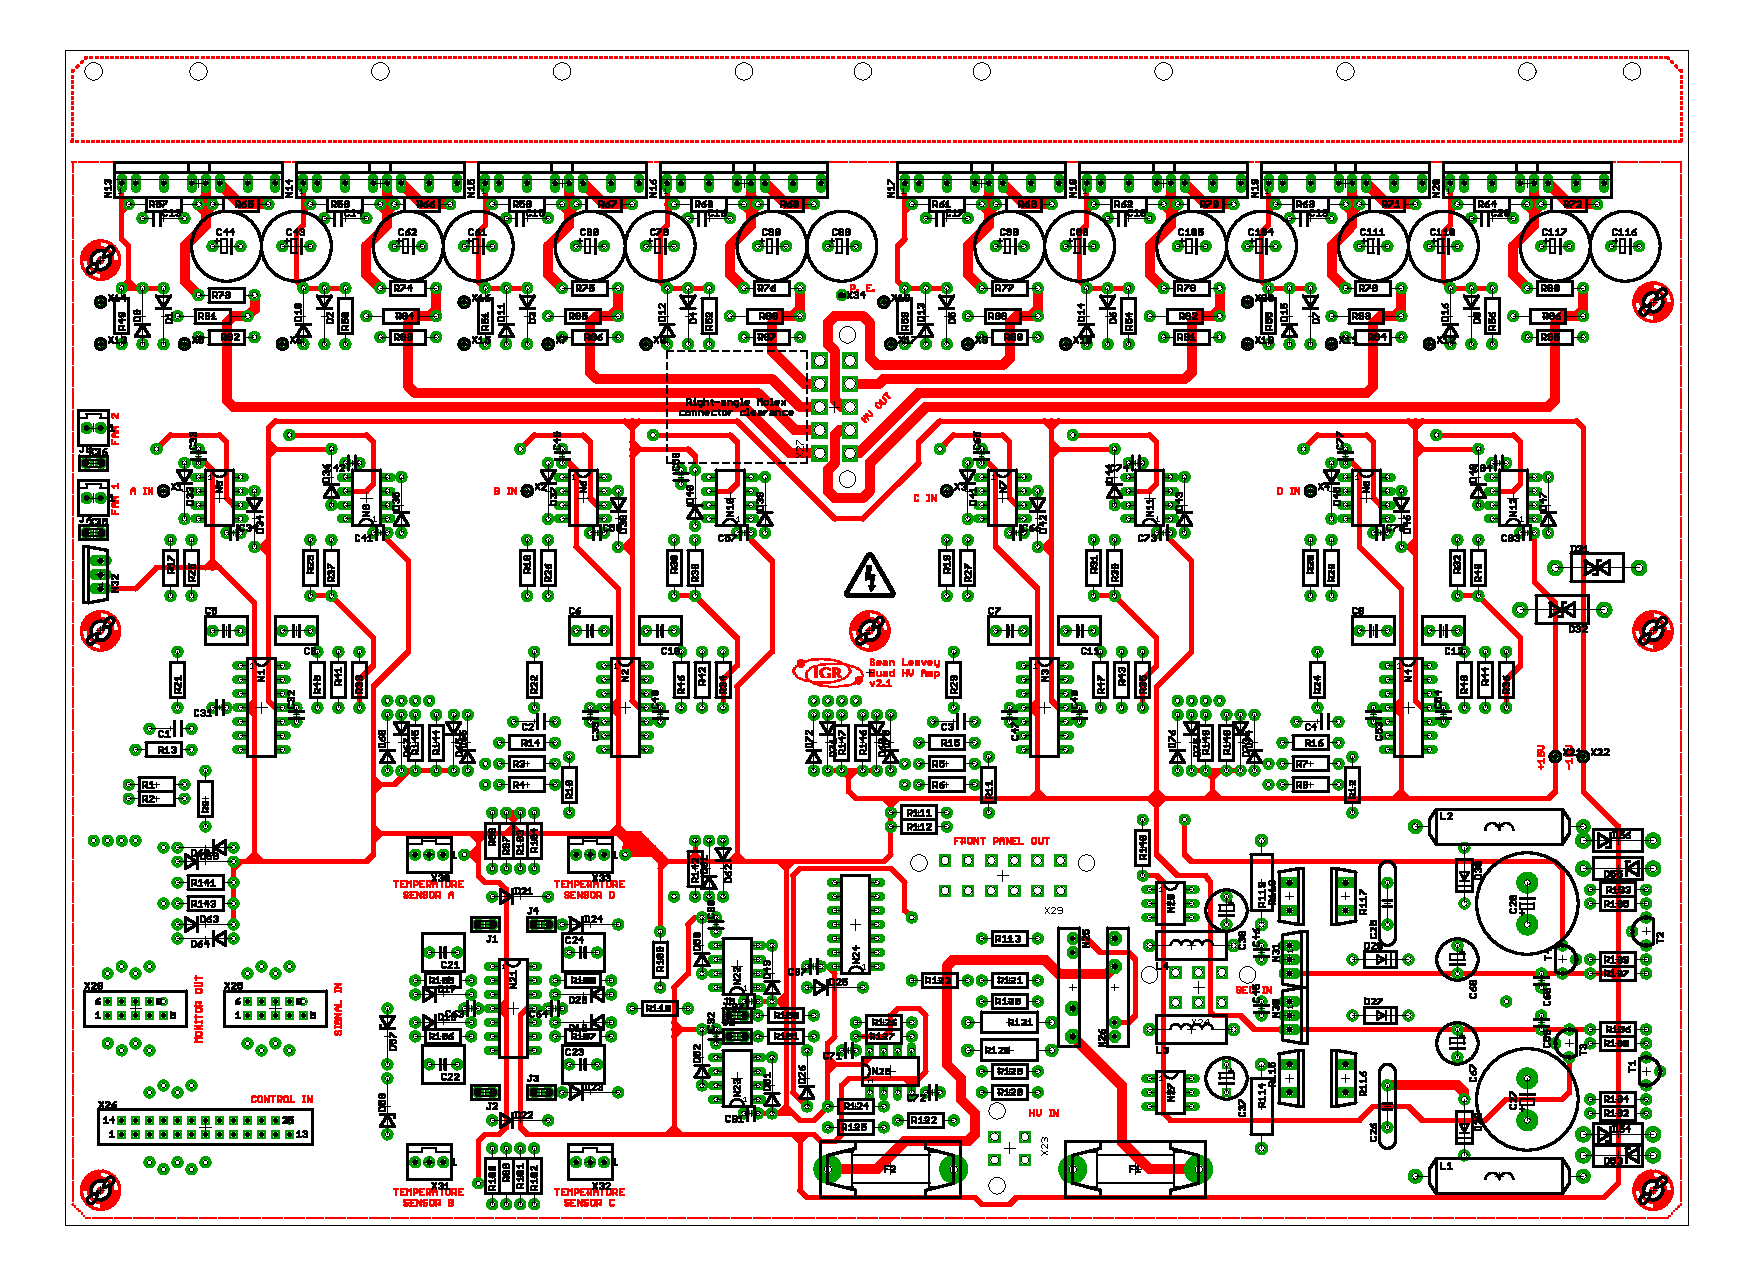
\includegraphics[width=\columnwidth]{graphics/60-hv-amp-top.pdf}
  \caption[High voltage amplifier board layout (top)]{\label{fig:hv-amp-top}Top view of the high voltage amplifier printed circuit board. In the lower left corner there are IDC connectors for the signal and control inputs and the monitor outputs. These connect via ribbon cables to the inside of the amplifier enclosure's front panel. Various other sockets are present in the lower half and upper centre of the board for high and low voltage inputs and outputs. The eight PA95 amplifier ICs are situated near the top of the board, and some space is left at the top of the board to allow these amplifiers to be attached to heat sinks. The copper layer immediately below the heat sink locations is isolated from the board's main ground plane to prevent the heat sinks from shorting the board's ground to earth. The bottom view is shown in Figure\,\ref{fig:hv-amp-bottom}.}
\end{figure}

\begin{figure}
  \centering
  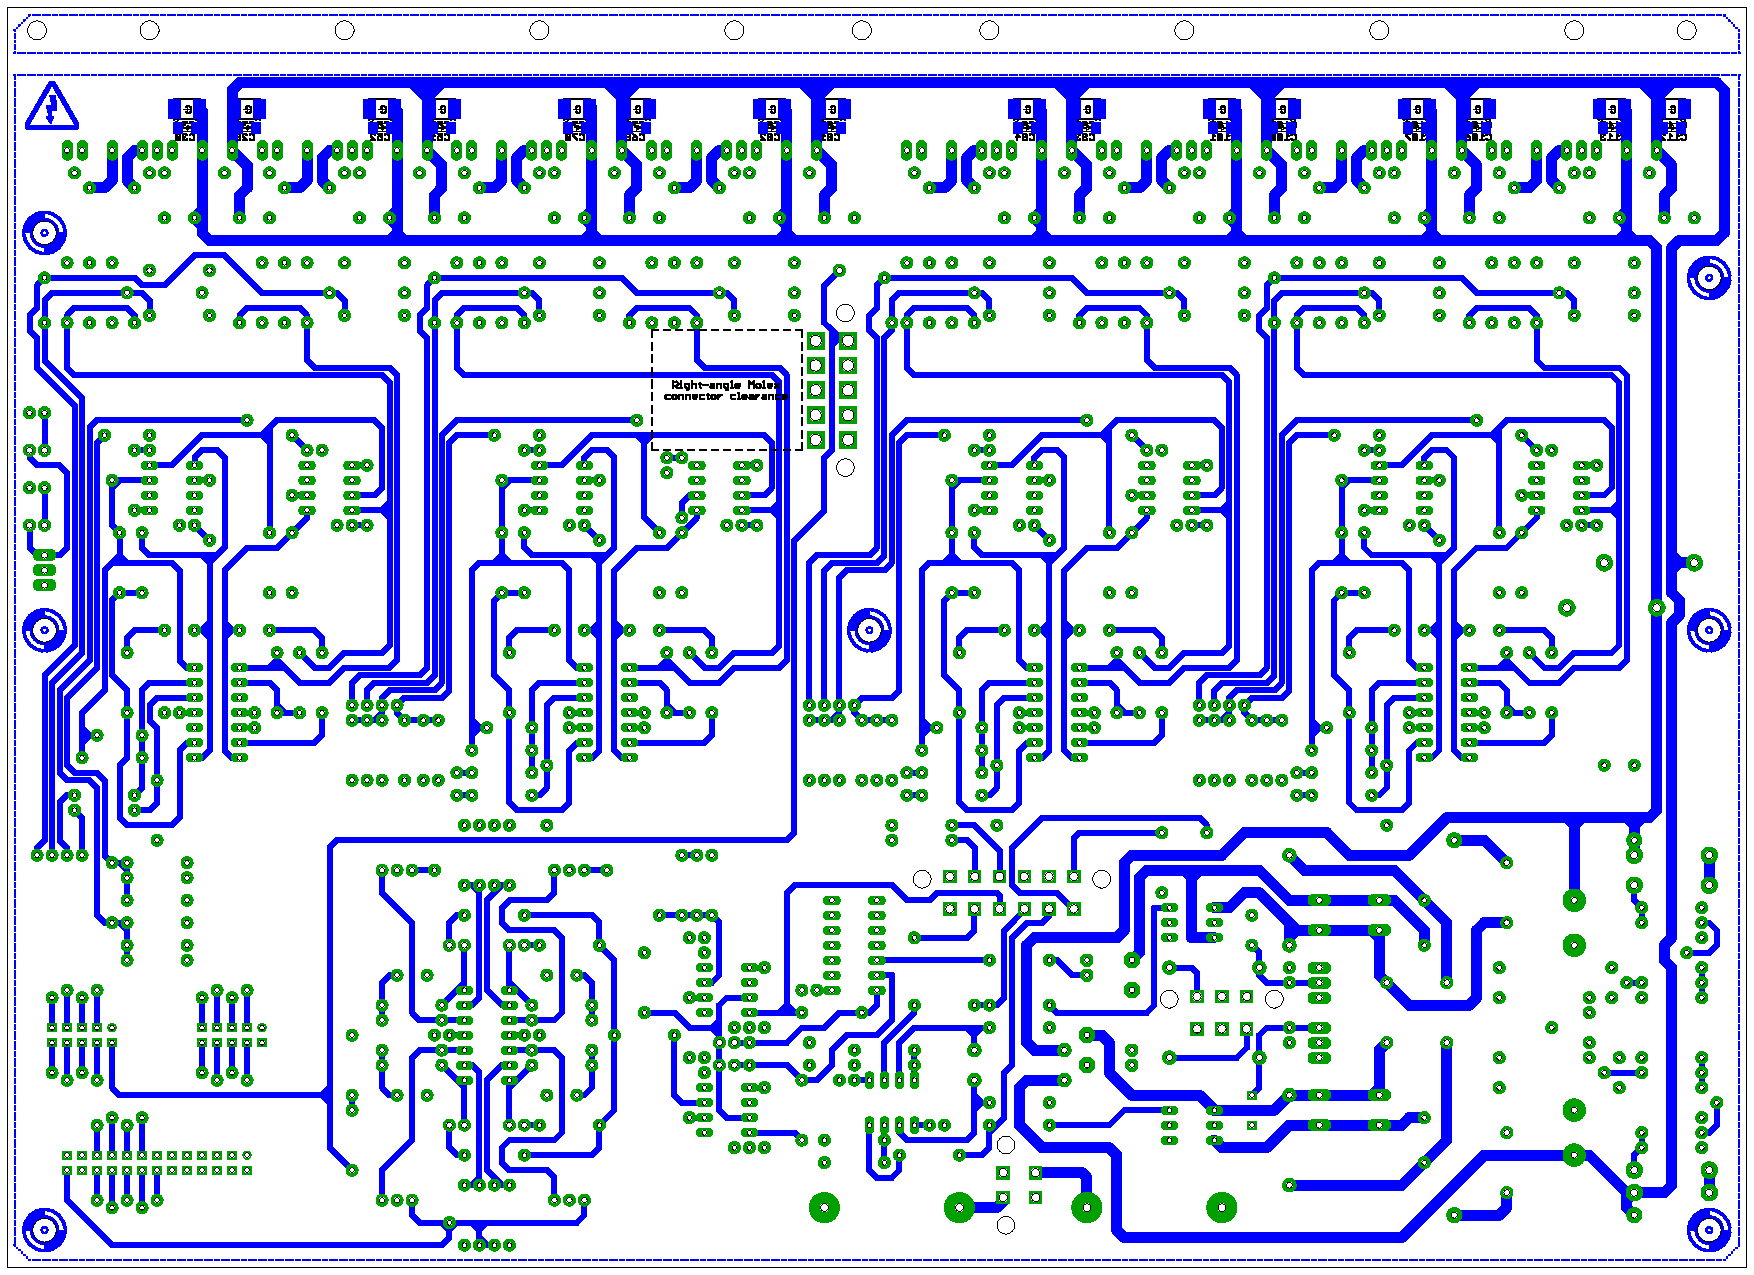
\includegraphics[width=\columnwidth]{graphics/60-hv-amp-bottom.pdf}
  \caption[High voltage amplifier board layout (bottom)]{\label{fig:hv-amp-bottom}Bottom view of the high voltage amplifier printed circuit board. The lower right corner of the board contains the ``soft start'' circuitry to charge the high voltage capacitors on the board, and the high voltage supply rails are routed from here to the top of the board where they are fed to each of the eight PA95 ICs. The remaining tracks on the bottom are predominantly used for board signal routing. The top view is shown in Figure\,\ref{fig:hv-amp-top}.}
\end{figure}

\begin{figure}
  \centering
  \includegraphics[width=\columnwidth]{graphics/generated/from-python/60-new-amplifier-dewhitened-tfs.pdf}
  \caption[Frequency response of the high voltage amplifier's channels with dewhitening enabled]{Second amplifier transfer functions with dewhitening enabled. The expected performance of the dewhitening filter from theory is shown in \checkme{green} alongside the transfer functions of each channel. The curves agree closely, showing that the implemented filter operates as expected. The mismatch at high frequency is caused by the anti-aliasing filters implemented in CDS, which aggressively filter signals above \checkme{a few \SI{}{\kilo\hertz}} (\note{see Chapter 4 AA filter section}).}
  \label{fig:new-amplifier-dewhitened-tfs}
\end{figure}

\begin{figure}
  \centering
  \includegraphics[width=\columnwidth]{graphics/generated/from-python/60-new-amplifier-channel-one-tfs.pdf}
  \caption[]{}
  \label{fig:new-amplifier-dewhitened-tfs}
\end{figure}

\begin{figure}
  \centering
  \includegraphics[width=\columnwidth]{graphics/generated/from-python/60-new-amplifier-coherence.pdf}
  \caption[High voltage amplifier cross-channel coherence]{Second amplifier channel coherence.}
  \label{fig:new-amplifier-coherence}
\end{figure}

\section{Experimental test of the electrostatic drive}
To set requirements on the positioning of the plates, and to build and test the infrastructure for the operation of the \glspl{ESD}, this chapter introduces the design for an experiment to test the new \gls{ESD} design.

\begin{table}
  \centering
  \begin{tabular}{ll}
    \textbf{Parameter}   & \textbf{Value} \\
    Mirror diameter      & \SI{30}{\milli\meter} \\
    Mirror thickness     & \SI{6}{\milli\meter} \\
    Single plate width   & \SI{30}{\milli\meter} \\
    Single plate length  & \SI{50}{\milli\meter} \\
    Nominal plate separation & \SI{40}{\milli\meter} \\
  \end{tabular}
  \caption[Plate capacitor and optic parameters for the experiment to test the electrostatic drives for the \SSM{}]{\label{tab:esd-expt-parameters}Plate capacitor and optic parameters for the experiment to test the electrostatic drives for the \SSM{}.}
\end{table}

Although the \gls{ESD}, and indeed the \SSM{} experiment, primarily require corrections at lower frequencies where seismic noise is dominant, it is beneficial to utilise an amplifier which can provide actuation up to many tens, if not hundreds, of \SI{}{\kilo\hertz}. This facilitates a transfer function which is flat across the vast majority of each experiment's measurement band, avoiding the roll-off at high frequencies due to the integrated circuits utilised within the high voltage amplifier. A flat transfer function makes the calibration of the actuator plant as part of the overall experiment as simple as possible. Another benefit of having a high bandwidth amplifier is the possibility to use it for common mode control loops, where laser frequency stabilisation can be split between feedback to the laser's piezoelectric transducer and actuators on the test masses.

The key component of a high bandwidth amplifier is the power op-amp. This class of op-amps typically utilises a \gls{MOSFET} design, and can provide high voltage output given a low voltage input. As an example, the Apex PA95 op-amps used in Advanced LIGO's \glspl{ESD} provide up to \SI{900}{\volt} output up to a frequency of around \SI{15}{\kilo\hertz}, and up to \SI{50}{\volt} at \SI{250}{\kilo\hertz}. The PA98 op-amp, also from Apex, provides an output of \SI{450}{\volt} nominally up to \SI{60}{\kilo\hertz}, potentially up to \SI{500}{\kilo\hertz} for a low capacitive load. For the purposes of this experiment, the choice was made to use the PA98 op-amp to provide the ability to study the effect of the actuator across a very wide bandwidth. To this end, an amplifier circuit utilising the PA98 was built based on a design used for the \AEIPROTOTYPE{}. This design provides up to \SI{\pm350}{\volt} output, and originates from a single-ended, \SI{350}{\volt} amplifier design where the PA98 is especially suited. Two notable modifications have been made, with a view to safety.

% claim about voltage output of PA95 comes from figure ``Power Response'' on p3 of PA95 datasheet (https://www.apexanalog.com/resources/products/pa95u.pdf)
% claim about voltage output of PA98 comes from figure 8: ``power Response'' on p7 of PA98 datasheet (https://www.apexanalog.com/resources/products/pa98u.pdf)

\section{Outlook}